\documentclass[a4paper]{article}
\usepackage[margin=1cm]{geometry}
\usepackage{booktabs}
\usepackage{array}
\usepackage{xcolor}
\usepackage{tikz}
\usetikzlibrary{shapes.geometric, arrows.meta, positioning, calc, matrix, shadows, fit, backgrounds}
% Whitepaper palette (soft academic pastels)
\definecolor{pBlue}{RGB}{210,230,245}
\definecolor{pGreen}{RGB}{210,236,220}
\definecolor{pYellow}{RGB}{255,244,220}
\definecolor{pOrange}{RGB}{255,220,200}
\definecolor{pPurple}{RGB}{232,226,242}
\definecolor{pGray}{RGB}{232,232,236}
\definecolor{pRose}{RGB}{245,220,222}
\definecolor{pLavender}{RGB}{232,226,242}
\definecolor{pSky}{RGB}{210,230,245}
\definecolor{pMint}{RGB}{210,236,220}
\definecolor{pCream}{RGB}{255,244,220}
\definecolor{pPeach}{RGB}{255,220,200}
\definecolor{pFog}{RGB}{232,232,236}
\definecolor{dpBlue}{RGB}{110,155,205}
\definecolor{dpOrange}{RGB}{230,150,95}
\tikzset{
  card/.style={
    rectangle, rounded corners=5pt,
    draw=black!70, line width=0.55pt,
    drop shadow={shadow xshift=1pt, shadow yshift=-1.2pt, fill=black, opacity=0.12},
    align=left, inner sep=7pt, font=\small
  },
  innercard/.style={
    rectangle, rounded corners=3pt,
    draw=black!55, line width=0.45pt, dashed,
    align=left, inner sep=5pt, font=\footnotesize
  },
  chip/.style={
    rectangle, rounded corners=3pt,
    draw=black!55, line width=0.4pt,
    align=center, inner sep=4pt, font=\scriptsize
  },
  flowarrow/.style={-{Latex[length=4.5pt]}, black!80, line width=0.65pt},
  arrow/.style={-{Latex[length=4.5pt]}, black!80, line width=0.65pt},
  decision/.style={
    diamond, aspect=2.2, draw=black!70, line width=0.55pt,
    drop shadow={shadow xshift=1pt, shadow yshift=-1.2pt, fill=black, opacity=0.12},
    align=center, inner sep=2pt, font=\small\bfseries, fill=pCream
  }
}
\pagestyle{empty}
\begin{document}
\noindent
% Standalone source. Rebuild commands are in README.md.
% Whitepaper palette and styles are embedded below and above.
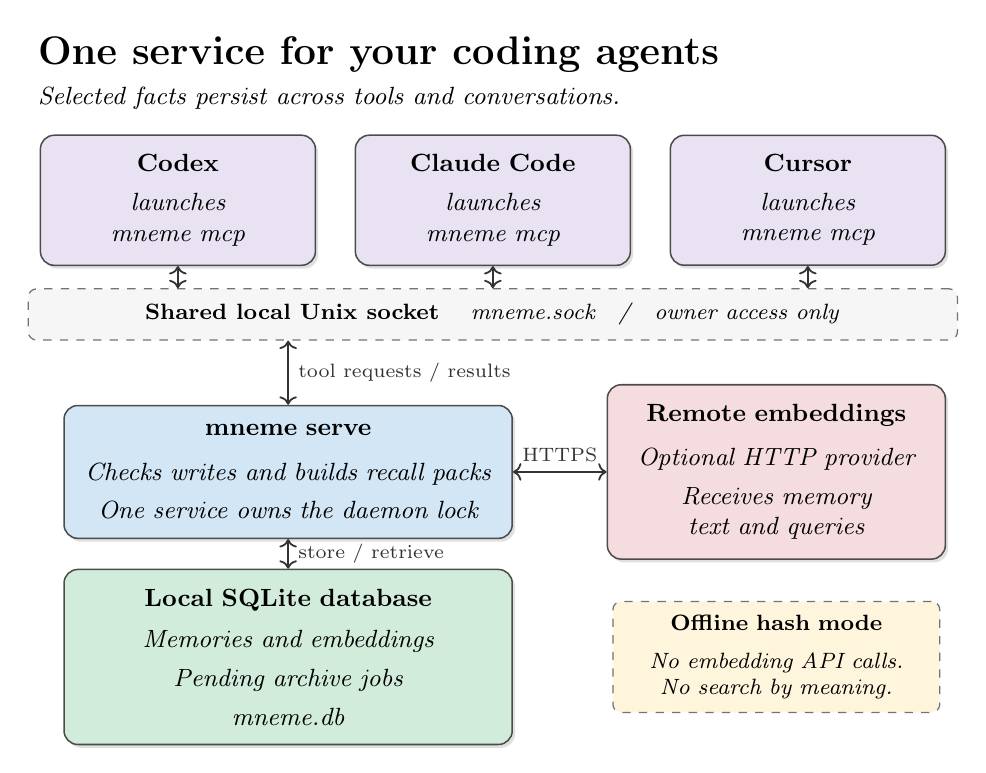
\begin{tikzpicture}
\node[font=\Large\bfseries, anchor=west] at (-5.9,7.1) {One service for your coding agents};
\node[font=\small\itshape, anchor=west] at (-5.9,6.55) {Selected facts persist across tools and conversations.};
\node[card,fill=pLavender,text width=3.0cm,align=center] (codex) at (-4,5.25) {\textbf{Codex}\\[3pt]{\itshape launches mneme mcp}};
\node[card,fill=pLavender,text width=3.0cm,align=center] (claude) at (0,5.25) {\textbf{Claude Code}\\[3pt]{\itshape launches mneme mcp}};
\node[card,fill=pLavender,text width=3.0cm,align=center] (cursor) at (4,5.25) {\textbf{Cursor}\\[3pt]{\itshape launches mneme mcp}};
\node[innercard,fill=pFog!40,minimum width=11.8cm,minimum height=0.65cm,align=center] (socket) at (0,3.8) {\textbf{Shared local Unix socket} \quad \textit{mneme.sock \; / \; owner access only}};
\draw[flowarrow,<->] (codex.south) -- (codex.south |- socket.north);
\draw[flowarrow,<->] (claude.south) -- (socket.north);
\draw[flowarrow,<->] (cursor.south) -- (cursor.south |- socket.north);
\node[card,fill=pSky,text width=5.2cm,align=center,minimum height=1.4cm] (daemon) at (-2.6,1.8) {\textbf{mneme serve}\\[5pt]{\itshape Checks writes and builds recall packs}\\[3pt]{\itshape One service owns the daemon lock}};
\draw[flowarrow,<->] (socket.south -| daemon.north) -- node[right,font=\scriptsize]{tool requests / results} (daemon.north);
\node[card,fill=pMint,text width=5.2cm,align=center] (db) at (-2.6,-0.55) {\textbf{Local SQLite database}\\[4pt]{\itshape Memories and embeddings}\\[3pt]{\itshape Pending archive jobs}\\[3pt]{\itshape mneme.db}};
\draw[flowarrow,<->] (daemon.south) -- node[right,font=\scriptsize]{store / retrieve} (db.north);
\node[card,fill=pRose,text width=3.8cm,align=center,minimum height=1.5cm] (provider) at (3.6,1.8) {\textbf{Remote embeddings}\\[5pt]{\itshape Optional HTTP provider}\\[3pt]{\itshape Receives memory text and queries}};
\draw[flowarrow,<->] (daemon.east) -- node[above,font=\scriptsize]{HTTPS} (provider.west);
\node[innercard,fill=pCream,text width=3.8cm,align=center] at (3.6,-0.55) {\textbf{Offline hash mode}\\[4pt]\textit{No embedding API calls.}\\\textit{No search by meaning.}};
\end{tikzpicture}

\end{document}
